\chapter{Konzeptionierung}

Um eine präzise und effiziente Umsetzung dieser Arbeit zu gewährleisten, wird zu Beginn der Fokus auf eine durchgängig durchdachte Kozeptionierung gelegt. Dies beginnt bereits bei der Definition der Anforderungen mithilfe des Requirements Engineering. Die definierten auszuarbeitenden Punkte werden im Anschluss mithilfe des COCOMO bewertet.

Nachdem die einzelnen Punkte definiert und bewertet sind, wird eine möglichst effiziente und passende Architektur entworfen. Auf diese wird ausführlich eingegangen, indem die Idee hinter dem Aufbau erklärt wird, sowie auch durch ein UML-Diagramm dargestellt wird.

Im Anschluss werden auch einzelne Methoden vorgestellt, sowie alle Parameter die die Lösung beeinflussen beschrieben.

In einer heutigen Software-Architektur sind die SOLID-Prinzipien nicht mehr weg zu denken. Diese werden in der Architektur beachtet, umgesetzt und auch in dieser Arbeit beschrieben.

\section{Software Engineering}{
Innerhalb einer Software-Entwicklung - wie im vorliegenden Fall - gilt es immer zuerst eine gründliche Anforderungsanalyse durchzuführen, um sicherzustellen dass alle Anforderungen erfasst und dokumentiert sind. Ebenso müssen eventuelle unbewusste Anforderungen ebenso herausgefunden werden, wie mögliche Begeisterungsfaktoren.

Um eine zeitliche Einschätzung durchführen zu können bietet sich das \ac{COCOMO} an. Hierbei werden der Aufwand der Implementierung geschätzt und eine ungefähre Anzahl der Codezeilen angegeben. Aus dieser Zahl kann dann per Formel eine Implementierungszeit errechnet werden. 

	\subsection{Requirements Engineering}
	Zu den grundsätzlichen Anforderungen gehören eine performante Umsetzung einer Softwarelösung des \ac{TSP}, der Verwendung einer effizienten Implementierung des \ac{ACO} und die Entwicklung einer durchdachten Architektur.
	Diese generellen Eigenschaften lassen sich aufteilen in genauer spezifizierte Anforderungen, sowohl aus funktionaler Sicht als auch aus nicht-funktionaler Sicht. Die funktionalen Anforderungen wären somit:
	\begin{itemize}
		\item Möglichkeit das \ac{TSP} lösen zu können
		\item Lösungsweg wird mit \ac{ACO} berechnet
	\end{itemize}
	Diese Arbeit beschränkt sich somit rein mit der Thematik das TSP möglichst effizient und performant zu lösen. Allerdings gibt es hier auch Einschränkungen betreffend auf die Umsetzung in Form der nicht-funktionalen Anforderungen, die wie folgt lauten:		
	\begin{itemize}
		\item Beachtung der ökonomischen Aspekte
		\item Objektorientierte Software
		\item Schnittstelle zum Erzeugen von Log-Daten
		\item Schnittstelle zum Einlesen von Problemdaten
		\item Berücksichtigung der SOLID-Prinzipien
		\item Auswahl leistungsfähiger Datenstrukturen
		\item Lesbarer, dokumentierter Sourcecode
		\item Lösungsqualität von 95%
		\item Programmiersprache: Java 8
		\item Zugelassene externe Bibliotheken: JUnit, HSQLDB
	\end{itemize}
	
	\newpage
	\subsection{COCOMO}
	Um eine wirtschaftliche Analyse in Bezug auf das vorliegende Softwareprojekt durchführen zu können, wird das \ac{COCOMO} angewendet. Hierbei wird die Funktionspunkt-Methode angewendet, da ein Implizieren der Anzahl der Codezeilen nicht verlässlich möglich ist. Hierzu werden die verschiedenen Teile der Architektur nach der Komplexität bewertet und aufgeteilt. Daraus ergibt sich folgende Liste:
	\begin{table}[H]
		\centering
		\footnotesize
		\setstretch{0.75}
	\begin{tabular}{l | c | c}
		\textbf{Komponente} & \textbf{Komplexität} & \textbf{Funktionspunkte} \\ \hline
		Externe Eingaben & Niedrig & 3 \\ \hline
		Externe Ausgaben & Niedrig & 4 \\ \hline
		Externe Anfragen & Hoch & 6 \\ \hline
		Externe Schnittstellen & Niedrig & 5\\ \hline
		Interne Logiken & Mittel & 10\\
	\end{tabular}
	\caption{Komplexitätseinschätzung des Projekts im Rahmen einer Abschätzung der Funktionspunkte}
	\end{table}
	Somit ergeben sich als Summe der Anforderungen an die Software 28 Funktionspunkte. In der verwendeten Programmiersprache Java entspricht ein Funktionspunkt im Durchschnitt ca. 53 Zeilen Code. Somit ergibt sich als Zeilenanzahl eine erwartete Menge von 1484 Zeilen. Mithilfe der ``\ac{COCOMO} II''-Formel lässt sich mit der Anzahl der Zeilen eine Arbeitsaufwand berechnen:
	\begin{equation}\label{cocomo}
		Aufwand = C * (Size)^{Prozessfaktoren} * M
	\end{equation}
	\begin{conditions*}
		C & Konstante\\
		Size & Anzahl der Codezeilen\\
		Prozessfaktoren & Kombinierte Prozessfaktoren\\
		M & Leistungsfaktoren\\
	\end{conditions*}
	\myequations{\ac{COCOMO} II-Formel zur Berechnung der Arbeitsaufwände bei der Entwicklung \& Implementierung eines Software-Projekts}
	Nach dieser Formel beträgt der zeitliche Aufwand für dieses Projekt ca. 2.5 Monate. Diese Zahl ist entsprechend einer Dauer eines Semesters von drei Monaten nachvollziehbar. Somit lässt sich auch sagen, dass das Projekt durchführbar ist und auch einen ausreichend großen Anspruch besitzt, um eine zu kurze Beschäftigungszeit zu verhindern.
}
\section{Architektur}{
	Die Architektur wurde inhaltlich so aufgeteilt, dass eine modulare Implementierung möglich ist. So wurden die vier folgenden Bereiche definiert: Persistenz, Applikation, TSP und ACO
	
	Der Begriff der Persistenz beschreibt in diesem Fall zusätzlich zum dauerhaften Abspeichern der Daten, auch das Einlesen der verschiedenen Problemstellungen.
	\newline
	Applikation umfasst den Teil des Programms, der sich nicht direkt mit Daten befasst aber auch nicht zur Problemlösung beiträgt, wie die zwei folgenden Bereiche.
	\newline
	Innerhalb des Begriffs TSP werden alle nötigen Parameter und Methoden behandelt, die basierend auf dem Traveling Salesman Problem notwendig werden. 
	\newline
	Zuletzt gibt es in der Architektur noch das Feld ACO, welches die komplette Berechnung des zu lösenden Problems übernimmt. In dem Fall, dieser Arbeit handelt es sich um das TSP. Allerdings könnte das Problemfeld auch dadurch ausgewechselt werden, dass der Bereich TSP um das neue Problem ersetzt wird.
	
	\subsection{Persistenz}
	Um ein starres Definieren des Problems innerhalb der Applikation zu verhindern, werden zu Beginn des Programms alle Parameter, wie Städtematrix, Wahrscheinlichkeiten und Lösungsparameter aus einer gegebenen XML-Datei eingelesen. Durch eine Bearbeitung der XML ist ein einfaches Abändern der Problemstellung möglich. Hierdurch ist auch gesichert, dass die Algorithmen effizient getestet werden können, da mehrere verschiedenen bekannte Testwerte benannt werden können.
	
	\subsection{Applikation}
	Wie bereits genannt, liegt bei der vorliegenden Architektur ein Fokus auf Modularität, Portabilität und Usability. Aber auch auf verlässliche und effiziente Algorithmen muss geachtet werden. Daher wird für die Wahrscheinlichkeitsberechnung die externe Klasse MersenneTwisterFast \footnote{s. http://www.math.sci.hiroshima-u.ac.jp/~m-mat/MT/emt.html} genutzt, welche eine bessere Distribution der Pseudozufallszahlen bieten als die Default-Implementierung in Java.
	\footnote{Um eine einfache und schnelle Benutzung zu gewährleisten, wird in dieser Arbeit darauf verzichtet echte Zufallszahlen zu nutzen, die beispielsweise aus Weltallstrahlung berechnet werden. Diese seien hier nur zur Vollständigkeit halber erwähnt.}
	Ein weiterer Bestandteil des Applikationsbereichs werden das Logging der Arbeitsvorgänge, sowie die zentrale Konfiguration der Problemstellung auf der die Lösung basiert.
	
	\subsection{TSP}
	Der Bereich des TSP definiert sich in dieser Architektur rein durch die Städte-Objekte, welche zur Darstellung der Städtematrix genutzt werden. Der einzige andere Bestandteil ist die zentrale Aufstellung der Städtematrix, die von den restlichen Klassen nur kopiert wird.
	
	\subsection{ACO}
	Um den Ameisenalgorithmus umzusetzen sind deutlich mehr Aufwände nötig, als zur Darstellung des TSP. Hier werden mindestens eine Ameisenkolonie benötigt \footnote{Die Architektur würde bei ausreichenden Systemressourcen auch eine parallele Berechnung mehrerer Städtematrizen erlauben},
	sowie je Kolonie mehrere Ameisen.
	\newline
	Die Ameisen werden in der Applikation als einzelne Threads gestartet, die über eine CyclicBarrier kontrolliert werden. Dies erlaubt ein möglichst effizientes Parallelisieren der Lösung.
	
	\subsection{Arbeitsweise der Architektur}
	Die einzelnen Abschnitte der Architektur wurden bereits erklärt. Aber das Zusammenspiel der einzelnen Komponenten und der eigentliche Arbeitsablauf des Systems wurde noch nicht beschrieben. Im Folgenden wird ein Beispiel so durchgeführt, wie es auch die geplante Architektur umsetzen würden.
	\begin{figure}[h]
		\centering
		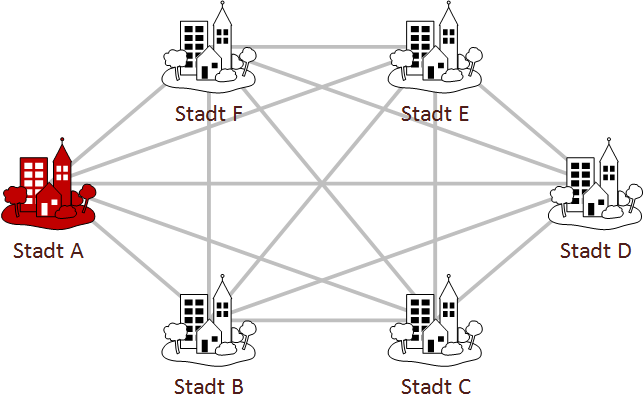
\includegraphics[width=0.9\linewidth]{images/TSP_ACO_numerisch.png}
		\caption{Darstellung des TSP-Beispiels zur Darlegung der Arbeitsweise der Architektur}
		\label{tspAcoNumerisch}
	\end{figure}
}
\section{UML-Diagramm}{

}
\section{Umsetzung der SOLID-Prinzipien}{
	Um eine saubere und übersichtliche Implementierung gibt es heutzutage eine Vielzahl von Regelwerken, Anleitungen und Vorgaben. Eine Sammlung von Grundsätzen sind die SOLID-Prinzipien. SOLID steht für \textbf{S}ingle Responsibility, \textbf{O}pen/Closed, \textbf{L}iskov Substitution, \textbf{I}nterface Segregation und \textbf{D}ependency Inversion.
	Alle diese Eigenschaften werden im Folgenden kurz erklärt und dann ihre Verwirklichung in der Architektur gezeigt.
	
	\subsection{Single Responsibility}
	Das Single-Responsibility-Prinip umschreibt den Zustand, dass Klassen max. eine Zuständig haben sollen. Klassen dürfen nicht mehrere Aufgabengebiete gleichzeitig übernehmen, da hierdurch eine Änderung an dieser Klasse zu einer Änderung mehrerer Komponenten führt und dadurch die ganze Struktur beeinflusst werden kann.
	Stattdessen wird die Software in mehrere kleinere Klassen aufgeteilt, die jeweils einen Teil übernehmen. Hierdurch ist zum Einen die Struktur einfacherer erkennbar und nachvollziehbar, da die Klassen eindeutiger definiert sind und der Code besser zusammengefasst ist. Zum Anderen sind die Abhängigkeiten aber auch auf ein Minimum reduziert.
	
	In der vorliegenden Konzeption ist dieser Grundsatz dadurch erfüllt, dass die Berechnungslogik an die Ameisen ausgegliedert ist, welche selbst keine Manipulation vornehmen. Die Ameisenkolonie hingegen funktioniert nur als Quelle der Threads und behält einige wenige Kolonie-spezifische Attribute bereit, sonst nichts.
	Andere Anwendungen, wie das Logging, das Einlesen von Konfigurationsdateien und die Zufallszahlerzeugung wurde alle in getrennte Klassen ausgegliedert, die zentral in \textit{Configuration} initialisiert werden.
	
	\subsection{Open / Closed}
	Die Open-Closed-Eigenschaft, welche eine moderne Software besitzen muss, umschreibt den Umstand, dass ein möglichst modularer Aufbau genutzt wird. So sollen Klassen so aufgebaut sein, dass bei einer Erweiterung keine Änderung bestehenden Codes notwendig wird, sondern zum Beispiel über das Implementieren eines Interfaces die alten Strukturen genutzt werden können.
	Unterscheiden muss man hier zwischen einer Erweiterung und einer Änderung. Die Software muss nicht und soll auch nicht auf eine einfache Änderung ausgelegt sein. Der Code, welcher erfolgreich implementiert wurde, soll auch in seinem Funktionsumfang weiter genutzt werden. Die bestehenden Implementierungen müssen keine Schnittstellen zur einfach Änderung enthalten.
	
	Durch die Schlichtheit der entworfenen Architektur und den auf die Problemstellung zugeschnittenen Charakter ist eine Umsetzung des Open-Closed-Prinzips nur in geringem Umfang möglich. Alleine die Parser können hiernach umgesetzt werden, in dem ein Interface eingesetzt wird. Dadurch wird ermöglicht in Zukunft auch andere Datei-Typen akzeptieren zu können.
	In der restlichen Implementierung ist eine Umsetzung nicht hilfreich oder zweckdienlich.
	
	\subsection{Liskov Substitution}
	Die Substitutionsregel von Liskov besagt, dass es möglich sein sollte eine Klasse in einem beliebigen Aufruf auch durch eine Subklasse aus zu tauschen ohne den Programmablauf zu ändern.
	Folglich müssen entweder die Implementierung abgestimmt sein, dass ein Austauschen generell möglich ist. Dies ist aber meist nicht zweckdienlich.
	Andererseits ist es auch möglich, über eine abstrakte Klasse zu arbeiten, die für Methodenaufrufe benutzt wird. So wird der Programmablauf nicht durch unterschiedliche Klassentypen unterbrochen, sondern der Entwickler ist in der Pflicht die abstrakte Klasse entsprechend umzusetzen.
	
	Ähnlich zu der Open-Closed-Eigenschaft ist auch diese Leitlinie in dem vorliegenden Entwurf nur sehr schwierig umzusetzen. Da von einem Hineinquetschen von Regeln und Leitlinien in eine Architektur generell abzuraten ist, wurde auf eine Umsetzung der Substitutionsregel generell verzichtet.
	
	\subsection{Interface Segregation}
	Die Trennung der Interfaces zielt darauf ab, Klassen nicht dazu zu zwingen Methoden zu implementieren, die gar nicht benötigt werden. So müssen in den meisten Programmiersprachen alle Methoden eines Interfaces zwingend umgesetzt werden. Dies führt aber meist zu einer aufgeblähten Codestruktur, da unnötige Methoden implementiert werden müssen, aber nie benutzt werden.
	Indem man die Interfaces in kleine Interfaces unterteilt ist es möglich durch eine Implementierung von mehrerer Interfaces auf das gleiche Ergebnis zu kommen ohne den Zwang alle anderen Interface auch umzusetzen.
	
	Aufgrund des Mangels an Interfaces in der Codestruktur der hier behandelten Architektur ist auch diese Regel nicht umgesetzt. Sobald Interface allerdings zum Einsatz kommen, muss diese Regel umgesetzt werden.
	
	\subsection{Dependency Inversion}
	Die Abhängigkeitsumkehr-Regel besagt, dass Module auf höheren Ebenen nicht auf Module niederer Ebenen angewiesen sein dürfen. Ähnlich zu den anderen Richtlinien sollen auch hier abstrakte Klassen und Interface zur Abstraktion genutzt werden.
	Allerdings gibt es noch den Zusatz, dass Abstraktionen niemals von einer detaillierten Implementierung abhängen dürfen.

	Wie bei den anderen Interface-Umsetzungen ist auch hier eine Umsetzung nicht hilfreich bzw. möglich. Dennoch sei auch hier erwähnt, dass eine Benutzung der Regel zu einfacher zu wartenden Code führt.
}
\section{Parameteranalyse}{

}
\section{Ausgewählte Algorithmen}{
\label{algorithms}
	Bereits vorgestellt wurden die einzelnen Bestandteile der Architektur, sowie die Architektur als Gesamtbild gezeigt. Im Folgenden sollen beispielhaft die verwendeten Algorithmen thematisch vorgestellt werden. So werden die zentralen Methoden zur Berechnung der Iterationen aus Sicht der Ameisen vorgestellt, sowie auch das Verhalten der Pheromonänderung. Zusätzlich wird die Methode zum Töten einer Ameise beschrieben, welche in so gut wie keiner Implementierung zu finden ist.
	
	\subsection{Ant - iteration()}
	In dem \ref{parameter} wurde bereits die Berechnung beschrieben, die für jede neue Streckenauswahl von den Ameisen durchgeführt werden muss. Diese Berechnung wird in der Implementierung in der Iteration der Ameisen umgesetzt. Pro Durchgang bzw. Iteration wird also jede besuchbare, angrenzende Stadt betrachtet und auf Ihre Attraktivität untersucht. Überwiegt der Pheromonwert $\tau$, welcher über Alpha gewichtet ist, über dem heuristischen Faktor $\eta$, der mit Beta verrechnet wird, so wird die bisher von der Kolonie gewählten Strecke gewählt. Diese Berechnung wird für alle Städte berechnet und dann verglichen. Die im Vergleich attraktivste Strecke wird in diesem Zusammenhang dann gewählt.
	Nachdem eine Strecke gewählt wird, verteilt die Ameise auf der Strecke ihre Pheromone indem der Kolonie ein Pheromonwert mitgeteilt wird, welcher auf den bisherigen addiert werden muss.
	
	\subsection{Colony - killAnt()}
	Ebenfalls in dem in Abbildung \ref{uml_class} gezeigten UML-Diagramm erkennbar ist, dass die Ameisenkolonie die Möglichkeit besitzt einzelne Ameisen zu "töten". 
	Diese Methode sollte in einem einwandfreiem Programm keinerlei Verwendung finden, allerdings kann man sich nicht auf eine dauerhafte fehlerfreie Implementierung verlassen. Im Bereich der Software Tests ist dies durch das Prinzip "Fehlen von Fehlern" beschrieben. Dieses sagt aus, dass erfolgreiche Tests nur bestätigen, dass keine Fehler gefunden wurden. Es kann nicht ausgesagt werden, dass keine Fehler vorliegen.\footnote{vgl. \cite{bibid}}
	
	Denn die Methode hat die Funktion, im Falle des Fehlverhaltens eine Ameise aus der Liste der aktiven Ameisen bzw. Threads zu löschen und den Thread zu stoppen.
	Genutzt werden wird diese vor allem im Bereich der aufgefangenen Fehler innerhalb der Implementierung der Ameisen. Sollte eine aufgetretene Exception schwerwiegend und unlösbar sein, wird die Applikation automatisch die Funktion aufrufen.
	
	\subsection{Colony - updatePheromone()}
	Schon mehrfach erwähnt wurden die Pheromonwerte, die Pheromonmatrix, sowie die Pheromonverteilung. All diese Begriffe sind auf die Ameisenkolonie zurückzuführen. Denn diese enthält die Pheromonmatrix, die von den Ameisen zur Berechnung der Iteration benutzt wird. Um diese aktuell zu halten wird diese von jeder Ameise nach jeder Iteration upgedatet. 
	
	Dabei wird die Funktion \textit{updatePheromone} der Kolonie aufgerufen und ein neuer Wert übergeben. Die Kolonie schreibt diesen dann in die zentrale Matrix, sodass der neue Wert bei der nächsten Iteration allen Ameisen ersichtlich ist. Durch diesen gleichzeitig und unübersichtlichen Zugriff auf die Matrix, muss diese Funktion synchronisiert ablaufen um einen Datenverlust zu verhindern.
	
}
\section{Sensitivitätsanalyse}{

}